\documentclass[a4paper,twocolumn,10pt]{onepgnote1}

% Essential packages
\usepackage{fontspec} % For LuaLaTeX/XeLaTeX
\setmainfont{Latin Modern Roman}
\usepackage{amsmath,amssymb,dsfont}
\usepackage[margin=10pt]{geometry}
\usepackage{yhmath}
\usepackage{tikz}
\usepackage[a]{esvect}
\usepackage{pgfplots}
\pgfplotsset{compat=1.18}
\usetikzlibrary{calc,arrows.meta,positioning}
\usepackage{xcolor} % Only once, with dvipsnames if needed
\usepackage{colortbl,array}
\renewcommand{\arraystretch}{1.5}

% ToDo notes (disable for final)
\usepackage{xargs}
\usepackage[colorinlistoftodos,prependcaption,textsize=tiny]{todonotes}
\newcommandx{\unsure}[2][1=]{\todo[linecolor=red,backgroundcolor=red!25,bordercolor=red,#1]{#2}}
\newcommandx{\change}[2][1=]{\todo[linecolor=blue,backgroundcolor=blue!25,bordercolor=blue,#1]{#2}}
\newcommandx{\info}[2][1=]{\todo[linecolor=OliveGreen,backgroundcolor=OliveGreen!25,bordercolor=OliveGreen,#1]{#2}}
\newcommandx{\improvement}[2][1=]{\todo[linecolor=Plum,backgroundcolor=Red!55,bordercolor=Red,#1]{#2}}
\newcommandx{\thiswillnotshow}[2][1=]{\todo[disable,#1]{#2}}
\newcounter{todocounter}
\newcommandx{\todocount}[2][1=]{\stepcounter{todocounter}\todo[linecolor=YellowGreen,backgroundcolor=YellowGreen!25,bordercolor=YellowGreen,#1]{\thetodocounter: #2}}

% Watermark
\usepackage{draftwatermark}
\SetWatermarkText{©FS Mathematik Gymnasium Gröbenzell}
\SetWatermarkScale{0.3}
\SetWatermarkColor[gray]{0.75}

% tcolorbox for notes
\usepackage{tcolorbox}
\renewtcbox{\notebox}{colback=yellow, colframe=yellow, sharp corners, nobeforeafter, box align=base, size=tight}
\renewcommand\mynote{\notebox{Hinweis:}\ }

% Custom commands
\newcommand{\kariert}[3]{%
  \begingroup
    \footnotesize #1 \normalsize\newline
    \begin{tikzpicture}
      \draw[step=0.5cm,color=gray] (0,0) grid (#2 cm ,#3 cm);
    \end{tikzpicture}
  \endgroup
}

\begin{document}
% no header, no footer.
\pagestyle{empty}
\section{Analysis}
\subsection{Grundlagen:}
\begin{itemize}
\item Binomische Formeln\\
\begin{enumerate}
\item $(a+b)^2 = a^2+2\cdot a\cdot b + b^2$\\
\item $(a-b)^2 = a^2 -2\cdot a\cdot b + b^2$\\
\item $(a+b)(a-b) = a^2 - b^2$
\end{enumerate}
\item Potenzengesetze\\
\begin{enumerate}
\item $a^r \cdot b^r = (a\cdot b)^r$ und $\frac{a^r}{b^r} = \left(\frac{a}{b}\right)^r$\\
\item $a^r \cdot a^s = a^{r+s}$ und $ \frac{a^r}{a^s} = a^{r-s}$\\
\item $(a^r)^s = a^{r\cdot s}$\\
\item $a^{\frac{m}{n}} = \sqrt[n]{a^m} = (\sqrt[n]{a})^m$\\
\item $a^{-r} = \frac{1}{a^r}$
\end{enumerate}
\item Logarithmengesetze\\
\begin{enumerate}
\item $\log_a(b\cdot c) = \log_a(b) + \log_a(c)$\\
\item $\log_a(\frac{b}{c}) = \log_a(b) - \log_a(c)$\\
\item $\log_a(b^r) = r\cdot \log_a(b)$\\
\item $\ln(x) = \log_e(x) \longrightarrow \ln(e^x) =x $\\
\item $\operatorname{ld}(x) = \log_2(x)$\\
\item $\operatorname{lg}(x) = \log_{10}(x)$
\end{enumerate}
\end{itemize}
\subsection{Lineare Transformationen:}\\
Wir erhalten aus dem Graphen $G_f$ der Funktion f den Graphen der Funktion g mit:\\
\begin{enumerate}
    \item $g(x) = - f(x)$, indem man $G_f$ an der x--Achse spiegelt\\
\item $g(x) =f(-x)$, indem man $G_f$ an der y--Achse spiegelt\\
\item $g(x) = f(x) +a$ indem man $G_f$ in Richtung der y--Achse um a verschiebt\\
\item $g(x) =f(x-a)$ indem man $G_f$ in Richtung der x--Achse um a verschiebt\\
\item $g(x) =a\cdot f(x)$ und $a>0$, indem man $G_f$ in Richtung der y--Achse mit dem Faktor a streckt bzw. staucht\\
\item $g(x) =f(a\cdot x)$ und  $a>0$, indem man $G_f$ in Richtung der x--Achse mit dem Faktor $\frac{1}{a}$ staucht bzw. streckt.\\

\end{enumerate}

\subsection{Ableitungen:}\\
\begin{enumerate}
\item jede Ableitung ist mit der $h-$Methode nachweisbar $$f'(x) = \lim \limits_{h\longrightarrow 0} \frac{f(x+h) - f(x)}{h}$$
\item $f(x)= c$ mit $c \in\mathds{R} \longrightarrow f'(x) = 0$\hfill\\
\item $f(x)= x  \longrightarrow f'(x) = 1$\\
\item $f(x) = c\cdot x $ mit $c\in\mathds{R}\longrightarrow f'(x) = c$ \\
\item $f(x) = m\cdot x + t  \hspace{0.2cm}\text{mit} \hspace{0.2cm} m,t \in \mathds{R}\longrightarrow f'(x) = m$\\
\item $f(x) = a\cdot g(x)\hspace{0.2cm}\text{mit} \hspace{0.2cm} a \in \mathds{R} \longrightarrow f'(x) = a\cdot g'(x)$ \\
\item $f(x)= g(x) \pm h(x) \longrightarrow f'(x) = g'(x)\pm h'(x)$\\
\item $f(x) = x^n$ mit $n\in \mathds{Q} \longrightarrow f'(x) = n\cdot x^{n-1}$\\
\item $f(x) = g(x) \cdot h(x) \longrightarrow f'(x) = g'(x) \cdot h(x) + g(x) \cdot h'(x)$\\
\item $f(x) = g(h(x)) \longrightarrow f'(x) = g'(h(x)) \cdot h'(x)$\\
\item $f(x) = \dfrac{z(x)}{n(x)} \longrightarrow f'(x) = \dfrac{n(x)\cdot z'(x) - z(x) \cdot n'(x)}{(n(x))^2}$\\ Eselsbrücke\footnote{N-Nenner, Z-Zähler, AZ - Ableitung Zähler, AN - Ableitung Nenner} : $f'(x)=\dfrac{N\cdot AZ-Z\cdot AN}{N^2}$
\end{enumerate}
\subsection{Ableitung spezieller Funktionen:}
\begin{itemize}
\item Trigonometrische Funktionen\\
\begin{enumerate} \item $f(x)= \sin{x} \longrightarrow f'(x) = \cos(x)$\\
\item $f(x)= \cos(x) \longrightarrow f'(x) = -\sin(x)$\\
\item $f(x) = \tan(x)= \dfrac{\sin(x)}{\cos(x)}$ \\$ \longrightarrow f'(x) = \dfrac{\cos(x) \cdot \cos(x) + \sin(x) \cdot \sin(x)}{(\cos(x))^2} = \dfrac{1}{(\cos(x))^2}$
\end{enumerate}
\item e-Funktion\\ \begin{enumerate} \item $f(x) = e^x \longrightarrow f'(x) = e^x$ \\ \item $f(x) = e^{h(x) } \longrightarrow f'(x) = h'(x) \cdot e^{h(x)}$\end{enumerate}
\item ln-Funktion\\ \begin{enumerate} \item $f(x) = \ln(x)$ mit $x\in \mathds{R}^+ \longrightarrow f'(x) = \dfrac{1}{x}$ \end{enumerate}
\item Wurzel\\ \begin{enumerate}\item $f(x) = \sqrt{x} = x^{\frac{1}{2}} \longrightarrow f'(x) = \dfrac{1}{2} \cdot x^{-\frac{1}{2}} = \frac{1}{2\sqrt{x}}$\\ \item $f(x)= \sqrt[n]{x} = x^{\frac{1}{n}} \longrightarrow f'(x) = \frac{1}{n} \cdot x^{\frac{1}{n} -1} = \frac{1}{n\cdot \sqrt[{n-1}]{x}}$\end{enumerate}
\end{itemize}
\subsection{Anwendung der 1. Ableitung}
\begin{itemize}
\item Zusammenhang Steigung $m$ des Graphen $G_f$ einer Funktion $f$ an der Stelle $x_0 \in G_f$ mit der 1. Ableitung:\\
\begin{enumerate}
\item $f'(x_0) = m$\\
\item $\tan{(\alpha)} = m \longrightarrow \alpha = \tan^{-1}{(m)}$
\end{enumerate}
\item Tangentengleichung $y_T$ durch den Punkt $P(x_0|f(x_0)) \in G_f \\y_T = f'(x_0)\cdot(x-x_0) + f(x_0) $
\item Newton-Verfahren $\longrightarrow$ Iterationsverfahren zur Bestimmung von Nullstellen\\
\begin{enumerate}
    \item Startwert $x_0 \longrightarrow $ je näher an der NS desto besser\\
    \item $x_{n+1} = x_n - \frac{f(x_n)}{f'(x_n)}$
    
\end{enumerate}
\end{itemize}
\subsection{Grenzwerte spezieller Funktionen:}
\begin{itemize}
\item Ist $p(x)$ ein Polynom, so gilt $\lim \limits_{x\longrightarrow \infty} \frac{p(x)}{e^x} = 0 \longrightarrow e-$Funktion.
\item Ist $p(x)$ ein nicht konstantes Polynom, so gilt \\$\lim \limits_{x\longrightarrow \infty} \frac{\ln(x)}{p(x)} = 0 \longrightarrow ln-$Funktion.
\item Ist $p(x)$ ein Polynom ohne konstanten Summanden , so gilt \\$\lim \limits_{x\longrightarrow 0} (p(x)\cdot \ln(x)) = 0\longrightarrow ln-$Funktion.
\end{itemize}
\subsection{Funktionsklassen:}
\subsubsection{Lineare Funktionen} 
\begin{itemize}
\item Funktionsterm: $f(x) = m\cdot x +t$ mit $m\in \mathds{R}\setminus\{0\}$ und $t\in \mathds{R}$ 
  \begin{enumerate}
  \item $m$ – Steigung der Geraden
  \item $t$ – y-Achsenabschnitt
  \end{enumerate}
  \item Graph einer linearen Funktion ist eine Gerade 
  \item Berechnung der Steigung $ m=\frac{\Delta y}{\Delta x}$
  \item Berechnung des y-Achsenabschnittes t $\longrightarrow$ die Steigung $m$ und die Koordinaten eines Punktes $P(x_0|y_0)$ einsetzen und nach $t$ auflösen
\end{itemize}
\subsubsection{Quadratische Funktionen:}
\begin{itemize}
\item allgemeine Form:$f(x) = a\cdot x^2 + b\cdot x +c$ mit $a\in \mathds{R}\setminus \{0\}$ und $b, c \in \mathds{R}$
\item Graph: 
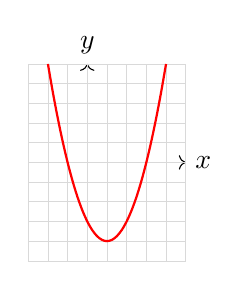
\begin{tikzpicture}[scale=0.25]
  % Achsen
  \draw[->] (-3,0) -- (5,0) node[right] {$x$};
  \draw[->] (0,-5) -- (0,5) node[above] {$y$};
  % Gitter
  \draw[very thin,color=gray!30] (-3,-5) grid (5,5);
  % Parabel: y = x^2 - 2x - 3
  \draw[thick,domain=-2:4,smooth,variable=\x,red] 
    plot ({\x},{\x*\x - 2*\x - 3});
\end{tikzpicture}
\item Scheitelpunktform: $f(x) = a\cdot(x-x_s)^2 +y_s$ mit $S(x_s|y_s)$ den Koordinaten des Scheitelpunktes
\item Faktorisierte Form: $f(x)= a\cdot (x-x_1)\cdot (x-x_2)$ mit $f(x_1)= 0$ und $f(x_2)= 0$ als Nullstellen der Funktion
\item Nullstellen als Lösung der Gleichung\\ $0 =a\cdot x^2 + b\cdot x +c \longrightarrow x_{1/2} = \dfrac{-b\pm\sqrt{b^2-4\cdot a\cdot c}}{2\cdot a}$
\item Für $a>0$ ist die Parabel nach oben geöffnet $\longrightarrow$ Scheitelpunkt ist Tiefpunkt und es gilt $
\lim\limits_{x \to \pm\infty} f(x) = \infty$
\item Für $a<0$ ist die Parabel nach unten geöffnet $\longrightarrow$ Scheitelpunkt ist Hochpunkt und es gilt $
\lim\limits_{x \to \pm\infty} f(x) = -\infty$\\[0.15cm]
\end{itemize}
\subsubsection{Polynome:}
\begin{itemize}
\item $f(x)= a_n\cdot x^n + a_{n-1} \cdot x^{n-1} + \cdots a_1 \cdot x + a_0 =\sum\limits_{i=0}^{n} a_i x^i$ mit $a_n\in \mathds{R}\setminus \{0\}$ und die restlichen $a_{i} \in \mathds{R}$
\item höchster Exponent legt den Grad des Polynoms fest $\longrightarrow$ hier $n-$ten Grades
\item Beispielgraphen in Abhängigkeit des Grades:\\
\begin{enumerate}\item a gerade: 
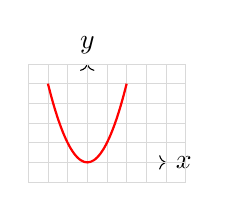
\begin{tikzpicture}[scale=0.25]
  % Achsen
  \draw[->] (-3,0) -- (4,0) node[right] {$x$};
  \draw[->] (0,-1) -- (0,5) node[above] {$y$};
  % Gitter
  \draw[very thin,color=gray!30] (-3,-1) grid (5,5);
  \draw[thick,domain=-2:2,smooth,variable=\x,red] 
    plot ({\x},{\x*\x});
\end{tikzpicture}
\item a ungerade: 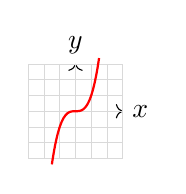
\begin{tikzpicture}[scale=0.2]
  % Achsen
  \draw[->] (-3,0) -- (3,0) node[right] {$x$};
  \draw[->] (0,-3) -- (0,3) node[above] {$y$};
  % Gitter
  \draw[very thin,color=gray!30] (-3,-3) grid (3,3);
     \draw[thick,domain=-1.5:1.5,smooth,variable=\x,red] 
    plot ({\x},{\x*\x*\x});
\end{tikzpicture}\\
\item $n$ gerade und $a_n > 0 \longrightarrow \lim\limits_{x \to \pm\infty} f(x) = \infty$\\
\item $n$ gerade und $a_n <0 \longrightarrow \lim\limits_{x \to \pm\infty} f(x) =- \infty$\\
\item $n$ ungerade und $a_n > 0 \longrightarrow \lim\limits_{x \to -\infty} f(x) = -\infty$ und $ \lim\limits_{x \to \infty} f(x) = \infty$\\
\item $n$ ungerade und $a_n < 0 \longrightarrow \lim\limits_{x \to -\infty} f(x) = \infty$ und $ \lim\limits_{x \to \infty} f(x) = -\infty$
\end{enumerate}
\item ab Grad $n>2$ kennen wir keine Lösungsformel zur Berechnung der Nullstellen\footnote{Für $n=2$ eist das Polynom eine Quadratischen Funktion} $\longrightarrow$ ausklammern bzw. Newton-Verfahren zur Näherung der Nullstellen
\end{itemize}
\subsubsection{Gebrochen-rationale Funktionen}
\begin{itemize}
\item $f(x) = \frac{z(x)}{n(x)}$ und $\mathds{D}_f = \mathds{R}\setminus\{x_i\}$ mit $n(x_i) = 0$
\item Definitionslücken sind die Nullstellen des Nennerpolynoms
\item Nullstellen berechnen sich durch  $0= z(x)$ sind also die Nullstellen des Zählerpolynoms
\item Graph $f(x) = \frac{x^2+1}{x-1} = x+1 +\frac{2}{x-1} $\\
 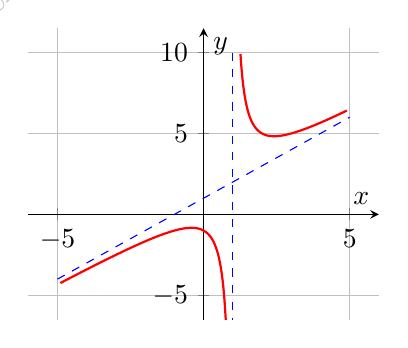
\begin{tikzpicture}
\begin{axis}[
    axis lines=middle,
    xmin=-5, xmax=5,
    ymin=-5, ymax=10,
    samples=400,
    domain=-4.9:4.9,
    restrict y to domain=-10:10,
    enlargelimits=true,
    xlabel={$x$}, ylabel={$y$},
    grid=both,
    scale= 0.65
]

% Die gebrochenrationale Funktion
\addplot[red, thick, domain=-4.9:0.9, unbounded coords=jump] {(x^2 + 1)/(x - 1)};
\addplot[red, thick, domain=1.1:4.9, unbounded coords=jump] {(x^2 + 1)/(x - 1)};

% Senkrechte Asymptote x = 1
\addplot[dashed, blue] coordinates {(1,-10) (1,10)};
% Schräge Asymptote: y = x + 1
\addplot[dashed, blue, domain=-5:5] {x + 1};
\end{axis}
\end{tikzpicture}\\
\mynote Bei der Monotonie- und Krümmungsuntersuchung muss die Definitionslücke explizit betrachtet werden, an der Definitionslücke kann sich das Monotonie- und Krümmungsverhalten ändern
\item Asymptoten: Die Art der Asymptote einer gebrochen-rationalen Funktion $f(x)=\frac{z(x)}{n(x)}$ mit $\mathds{D} = \mathds{D}_{\text{max}}$ hängt vom Grad der Polynome des Zählers  als auch des Nenners ab\footnote{z-Grad des Zählers; n - Grad des Nenners}.\\
\begin{enumerate}\item z $<$ n: die $x-$Achse ist waagerechte Asymptote $\lim\limits_{x\longrightarrow \infty} f(x) = \lim\limits_{x\longrightarrow -\infty} f(x) = 0$\\
\item  z $=$ n: waagerechte Asymptote die parallel zur x-Achse verläuft $\lim\limits_{x\longrightarrow \infty} f(x) = \lim\limits_{x\longrightarrow -\infty} f(x) = a \in\mathds{R}$\\
\item z $=$ n+1: schräge Asymptote die direkt aus der Summenform ablesbar ist \\
\mynote $f(x) =\underbrace{x+1}_{\shortstack{\text{Gleichung der}\\ \text{\textcolor{red}{schrägen} Asymptote}}} +\dfrac{2}{x-1}$\\
\item z $>$ n +1: Näherungskurve
\end{enumerate}
 \end{itemize}
 \subsubsection{$e-$Funktion:}
 \begin{itemize}
 \item $f(x) = e^x$
 \item Graph der Funktion $f(x)= e^x$\\
 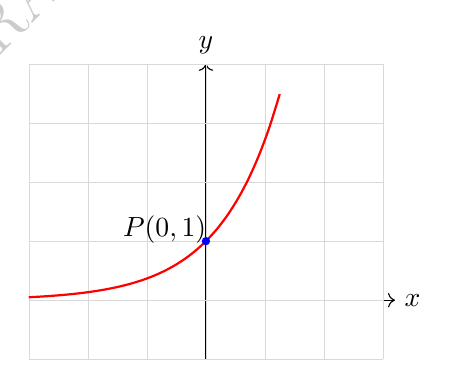
\begin{tikzpicture}[scale=0.75]
  % Achsen
  \draw[->] (-3,0) -- (3.2,0) node[right] {$x$};
  \draw[->] (0,-1) -- (0,4) node[above] {$y$};
  
  % Gitter
  \draw[very thin,color=gray!30] (-3,-1) grid (3,4);
  
  % Funktion e^x
  \draw[thick,domain=-3:1.25,smooth,variable=\x,red] 
    plot ({\x},{exp(\x)});
    % Punkt P(0,1)
  \fill[blue] (0,1) circle (2pt);  % Punkt P(0,1)
  \node at (-0.7,1.2) {$P(0,1)$};  % Beschriftung des Punktes
\end{tikzpicture}
\item Ableitung: $f'(x) = e^x$
\item Grenzwerte:\\
\begin{enumerate}
\item $\lim \limits_{x\longrightarrow -\infty} f(x) = 0$\\
\item $\lim \limits_{x\longrightarrow \infty} f(x) = \infty$
\end{enumerate}
\item $f(x) > 0: $ für alle $x\in \mathds{R}$\\
\mynote Die $e-$Funktion wächst schneller als jede Potenzfunktion $g(x)= x^n$ mit $n\in\mathds{N}$\\ \mynote Eselsbrücke: $e$ \textcolor{red}{gewinnt}!
\item Bei der Kurvendiskussion wird die $e-$Funktion meistens als Produkt mit einer anderen Funktion betrachtet.\footnote{$f(x) = g(x)\cdot e^{h(x)}  \longrightarrow f'(x) =g'(x)\cdot e^{h(x)} + g(x) \cdot h'(x) \cdot e^{h(x)} $}
 \end{itemize}
 \subsubsection{$ln-$Funktion:}
 \begin{itemize}
 \item $f(x) = \ln(x)$ mit $x\in \mathds{R}^+$
 \item Graph der Funktion $f(x)=\ln(x)$\\
 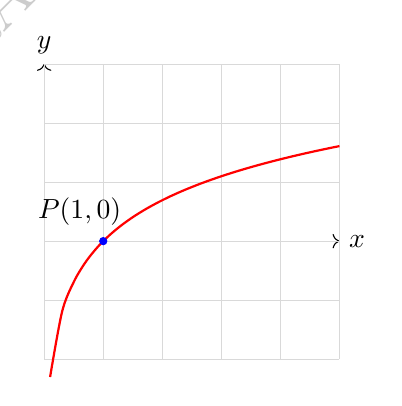
\begin{tikzpicture}[scale=0.75]
  % Achsen
  \draw[->] (0,0) -- (5,0) node[right] {$x$};
  \draw[->] (0,-2) -- (0,3) node[above] {$y$};
  
  % Gitter
  \draw[very thin,color=gray!30] (0,-2) grid (5,3);
  
  % Funktion ln(x)
  \draw[thick,domain=0.1:5,smooth,variable=\x,red] 
    plot ({\x},{ln(\x)});
  
  % Beschriftungen und Punkt (1, 0)
\fill[blue] (1,0) circle (2pt);  % Punkt P(0,1)
  \node at (0.6,0.5) {$P(1,0)$};  % Beschriftung des Punktes
\end{tikzpicture}
\item Ableitung $f'(x) = \frac{1}{x}$
\item Grenzwerte:\\
\begin{enumerate}
\item $\lim \limits_{x\longrightarrow 0^+} f(x) = -\infty$\\
\item $\lim \limits_{x\longrightarrow \infty} f(x) = \infty$
\end{enumerate}
\item \mynote Die $ln-$Funktion wächst langsamer als jede Potenzfunktion $g(x)= x^n$ mit $n\in\mathds{N}$,\\ \mynote Eselsbrücke: $\ln$ ist der \textcolor{red}{Loser}!
\item Bei der Kurvendiskussion wird die $ln-$Funktion meistens in Kombination mit einer anderen Funktion betrachtet.\footnote{$f(x) = \ln{(g(x))}  \longrightarrow f'(x) = \dfrac{1}{ g(x)} \cdot g'(x) = \dfrac{g'(x)}{g(x)} $}
 \end{itemize}
 \newpage
 \subsubsection{Wurzelfunktion:}
 \begin{itemize}
 \item $f(x) = a\cdot \sqrt{x-b}+c$ und $x\geq b$ ist eine Halbparabel und ergibt sich durch folgende lineare Transformationen aus der allgemeinen Wurzelfunktion $g(x)= \sqrt{x}$ wie folgt:\\
\begin{enumerate}
    \item Verschiebung um b in x-Richtung\\
    \item Strecken bzw. Stauchen mit dem Faktor a in y-Richtung\\
    \item Verschiebung um c in y-Richtung
\end{enumerate}
\item Graph der Funktion $f(x)= \frac{1}{2} \sqrt{x-2}+2$\\
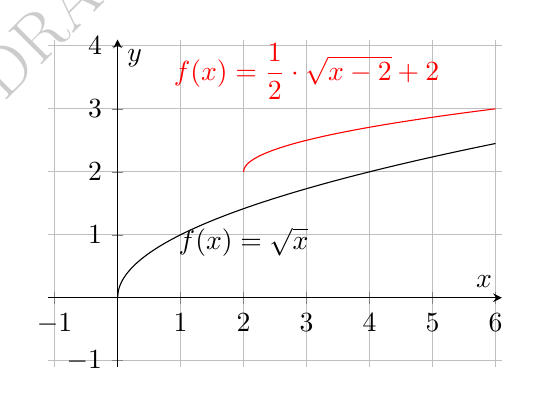
\begin{tikzpicture}
    \begin{axis}[xmin= -1.1, xmax = 6.1, ymin= -1.1, ymax=4.1,
    x=1cm,y=1cm,
        axis lines = middle, 
        ymajorgrids=true,
        xmajorgrids=true,
        xtick={-1,  ..., 6},
        ytick={ -1, ..., 4},
        xlabel = $x$,
        ylabel=$y$, 
        scale= 0.8]      

        \addplot[red, samples = 500, domain= 2:6]{2 + 0.5*(x-2)^(0.5)};
        \draw[red] (3,3)   node [above] {$f(x)=\dfrac{1}{2} \cdot \sqrt{x-2} + 2$};
        \addplot[ samples = 500, domain= 0:6]{(x)^(0.5)};
         \draw (2,0.5)   node [above] {$f(x)= \sqrt{x}$};
    \end{axis}
\end{tikzpicture}
\item Ableitung $f(x)= \sqrt{g(x)} \longrightarrow f'(x) = \frac{g'(x)}{2\cdot \sqrt{g(x)}}$
 \end{itemize}
 \subsubsection{allgemeine Sinusfunktion:} 
 \begin{itemize}
 \item $ f(x)= a\cdot \sin{(b\cdot (x - c))}+d $ mit  $a\in \mathds{R}\setminus\{0\}$ und $b,c,d \in \mathds{R}$
 \begin{enumerate}
\item Der Parameter $a$ ändert die Amplitute, also die maximale Auslenkung der Kurve.\\
\item Der Parameter b streckt bzw. staucht die Kurve in Richtung der x-Achse. Durch den Faktor b wird damit die Periode $p$ verändert $p = \frac{2\cdot \pi}{b}$.\\
        \item Der Parameter c verschiebt die Kurve in Richtung der x-Achse.\\
        \item Der Parameter d verschiebt die Kurve in Richtung der y-Achse.
 \end{enumerate}
 \item Ableitung: $f'(x)=  a\cdot \cos{(b\cdot (x - c))}\cdot b $
 \item Bei der Kurvendiskussion wird die $\sin-$Funktion meistens in Kombination mit einer anderen Funktion betrachtet.\footnote{$f(x) = \sin{(g(x))}  \longrightarrow f'(x) = \cos{(g(x))}\cdot g'(x) $}
 \end{itemize}
 \subsubsection{Betragsfunktionen:}
 \begin{itemize}
     \item Wird eine Funktion $g$ linaren Transformationnen in Form des Betrags unterworfen ergeben sich unterschiedliche Graphen. Diese Graphen haben allerdings gemeinsam, dass die Nicht-Differenzierbarkeit an bestimmten Stellen sich nicht ändert.\\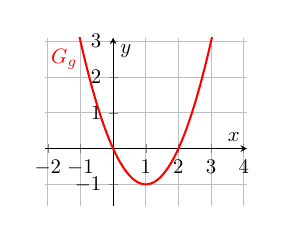
\begin{tikzpicture}[scale=0.75]
    \begin{axis}[xmin= -2.1, xmax = 4.1, ymin= -1.6, ymax= 3.1,
        axis lines = middle, 
        ymajorgrids=true,
        xmajorgrids=true,
        xtick={-2, ..., 4},
        ytick={-2, ..., 3},
        xlabel = $x$,
        ylabel=$y$, scale=0.5]
        \addplot[line width=1pt,mark=none, color=red]  plot[samples=300,smooth]{x^2-2*x};  
        \draw[red] (-1.5,2)   node [above] {$G_{g}$};       
    \end{axis}
\end{tikzpicture}
\item  $g_1(x) = |f(x)|:$ Die Punkte mit negativen Funktionswerten werden an der $x-Achse$ gespiegelt. Die Spiegelung erfolgt damit an den Nullstellen.\\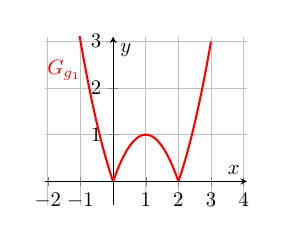
\begin{tikzpicture}[scale=0.75]
    \begin{axis}[xmin= -2.1, xmax = 4.1, ymin= -0.5, ymax= 3.1,
        axis lines = middle, 
        ymajorgrids=true,
        xmajorgrids=true,
        xtick={-2, ..., 4},
        ytick={-2, ..., 3},
        xlabel = $x$,
        ylabel=$y$, scale=0.5]
        \addplot[line width=1pt,mark=none, color=red, restrict x to domain=2:3]  plot[samples=900,smooth]{x^2-2*x}; 
   \addplot[line width=1pt,mark=none, color=red, restrict x to domain=-2:0]  plot[samples=900,smooth]{x^2-2*x};
    \addplot[line width=1pt,mark=none, color=red, restrict x to domain=0.000001:1.99999999999]  plot[samples=900,smooth]{-1*x^2+2*x};
        \draw[red] (-1.5,2)   node [above] {$G_{g_1}$};       
    \end{axis}
\end{tikzpicture}
\item $g_2(x) = f(|x|):$ Der im positive Teil der $x-Achse$ liegende Graaph wird an der $y-Achse$ gespiegelt.\\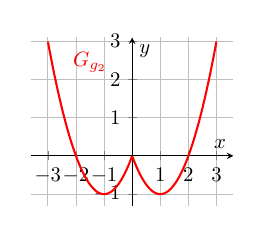
\begin{tikzpicture}[scale=0.75]
    \begin{axis}[xmin= -3.6, xmax = 3.6, ymin= -1.3, ymax= 3.1,
        axis lines = middle, 
        ymajorgrids=true,
        xmajorgrids=true,
        xtick={-3, ..., 4},
        ytick={-2, ..., 3},
        xlabel = $x$,
        ylabel=$y$, scale=0.5]
        \addplot[line width=1pt,mark=none, color=red, restrict x to domain=0:3]  plot[samples=900,smooth]{x^2-2*x}; 
   \addplot[line width=1pt,mark=none, color=red, restrict x to domain=-3:0]  plot[samples=900,smooth]{(-1*x)^2+2*x};
        \draw[red] (-1.5,2)   node [above] {$G_{g_2}$};       
    \end{axis}
\end{tikzpicture}
\item $g_3(x) = |f(|x|)|:$ Wird sowohl der Betrag der $x-Werte$ als auch der Betrag der Funktionswerte gebildet, werden zunächst die Punkte mit positiven $x-$Werten an der $y-$Achse gespiegelt um anschließend die Punkte mit negativen Funktionswerten an der $x-$Achse zu spiegeln.\\ 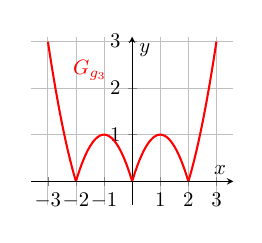
\begin{tikzpicture}[scale=0.75]
    \begin{axis}[xmin= -3.6, xmax = 3.6, ymin= -0.5, ymax= 3.1,
        axis lines = middle, 
        ymajorgrids=true,
        xmajorgrids=true,
        xtick={-3, ..., 4},
        ytick={-2, ..., 3},
        xlabel = $x$,
        ylabel=$y$, scale=0.5]
    \addplot[line width=1pt,mark=none, color=red, restrict x to domain=0:2]  plot[samples=900,smooth]{-1*x^2+2*x};
     \addplot[line width=1pt,mark=none, color=red, restrict x to domain=2:3]  plot[samples=900,smooth]{x^2-2*x}; 
    \addplot[line width=1pt,mark=none, color=red, restrict x to domain=-2:0]  plot[samples=900,smooth]{-1*x^2-2*x};
     \addplot[line width=1pt,mark=none, color=red, restrict x to domain=-3:-2]  plot[samples=900,smooth]{x^2+2*x}; 
        \draw[red] (-1.5,2)   node [above] {$G_{g_3}$};       
    \end{axis}
\end{tikzpicture}
 \item Betragsfunktionen sind an Knickstellen nicht differenzierbar $\longrightarrow$ Nachweis über die $h-$Methode.
 
 \end{itemize}
 \subsection{Kurvendiskussion:}\\
Bei der Kurvendiskussion werden Eigenschaften des Graphen $G_f$ einer Funktion $f$ analytisch untersucht
 \subsubsection{Untersuchung der Ausgangsfunktion:}
 \begin{itemize}
     \item Untersuchung folgender Eigenschaften:\\
     \begin{enumerate}
         \item Definitionsbereich $\longrightarrow$ bei gebrochen-rationalen Funktion z.B. Berechnung der Definitionslücken\\
         \item Schnittpunkte mit den Koordinatenachsen $\longrightarrow$ Nullstellen und Schnittpunkt mit der $y-$Achse\\
         \item Symmetrie zum Ursprung bzw. zur $y-$Achse\\
         \item Verhalten an den Rändern des Definitionsbereichs $\longrightarrow$ Grenzwerte und Verhalten an Definitionslücken\\
         \item Asymptoten
     \end{enumerate}
     \item je nach Funktionsklasse sind die Rechnungen unterschiedlich
 \end{itemize}
 \subsubsection{Monotonie:}
 \begin{itemize}
 \item Ist die Funktion $f$ im Intervall $I$ differenzierbar dann ist $G_f$ für  
 \begin{equation*}
	\left.\begin{aligned}
	f'(x) &>0  \\
	f'(x) &<0
	\end{aligned}
	\right\}
\quad \text{streng monoton}
	\quad\left\{\begin{aligned}
	\text{wachsend}\\
	\text{fallend}
	\end{aligned}
\right.
\end{equation*} 
\item \mynote Für die Existenz einer Extremstellen $x_0 \in G_f$ sind zwei Bedingungen notwendig:\\
\begin{enumerate} \item $f'(x_0)=0$\\
\item $f''(x_0) \neq 0$
\end{enumerate}
\item Die Art der einzelnen Extremstellen läßt sich leicht durch die Vorzeichenwechsel (VZW) der Ableitung an der Stelle $x_0$ mit $f'(x_0)=0$ bestimmen.
 \begin{itemize}
\item Hochpunkt (HoP) $HoP(x_0|f(x_0))$ genau dann, wenn es einen VZW der Ableitung von \textcolor{red}{positiv nach negativ} gibt. \begin{enumerate}\item $f'(x_0) = 0$\\ \item $f''(x_0) < 0$ \end{enumerate}
\item Tiefpunkt (TiP) $TiP(x_0|f(x_0))$ genau dann, wenn es einen VZW der Ableitung von \textcolor{red}{negativ nach positiv} gibt.  \begin{enumerate}\item $f'(x_0) = 0$\\ \item $f''(x_0) > 0$ \end{enumerate}
 \end{itemize}
 \item Untersuchung der Monotonie und der Extremstellen\\
 \begin{enumerate}
     \item Bestimmung der Nullstelle der 1. Ableitung\\
     \item Untersuchung der Monotonie mit Hilfe der Monotonietabelle\\
     \item Entscheidungen zu möglichen Extremstellen
 \end{enumerate}
 \item Monotonietabelle: Eintragung der Intervalle die durch die Nullstellen von $f'(x_1)= 0$ und $f'(x_2)=0$ festgelegt werden.\\
\mynote Beispiel mit zwei Nullstellen:\\\scalebox{0.75}{\begin{tabular}{||c|c|c|c|c|c||}
    \hline
    $x$& $ -\infty <x<x_1 $ & $ x =x_1$ &$ x_1<x<x_2 $ & $x =x_2 $& $ x_2<x<\infty $\\
    \hline \hline
    $f'(x)$ & + & 0 & - & 0 & +\\ 
    \hline
    $G_f$ & smw & $HoP$ & smf & $TiP$& smw\\
    \hline
\end{tabular}}
\item wenn sich das Monotonieverhalten \textcolor{red}{nicht} ändert, liegt ein \textcolor{red}{Terrassenpunkt} vor 
\item Bei gebrochen-rationalen Funktionen \textcolor{red} {muss die Definitionslücke in der Monotonietabelle ebenfalls betrachtet werden}.
 \end{itemize}
 \subsubsection{Krümmungsverhalten:}
 \begin{itemize}
     \item Der Punkt, an dem sich die Krümmung des Graphen der Funktion $f$ ändert, heißt Wendepunkt. 
     \item Am Wendepunkt des Graphen liegt ein Extremwert der lokalen Änderungsrate vor. 
     \item Ein Terrassenpunkt ist ein Wendepunkt mit einer waagerechten Tangente.
     \item Zusammenhang der lokalen Änderungsrate und der Krümmung:\\
     \begin{enumerate}
         \item Ist die Funktion $f$ im Intervall $I$ zweimal stetig differenzierbar und ist für alle $x\in I$ der Funktionswert $f''(x)$ \textcolor{red}{positiv}, dann ist der Graph der Funktion $f$ \textcolor{red}{linksgekrümmt}.\\
         \item Ist die Funktion $f$ im Intervall $I$ zweimal stetig differenzierbar und ist für alle $x\in I$ der Funktionswert $f''(x)$ \textcolor{red}{negativ}, dann ist der Graph der Funktion $f$ \textcolor{red}{rechtsgekrümmt}.
     \end{enumerate}
      \item Untersuchung der Krümmung und der Wendestellen\\
 \begin{enumerate}
     \item Bestimmung der Nullstelle der 2. Ableitung\\
     \item Untersuchung der Krümmung mit Hilfe der Krümmungstabelle\\
     \item Entscheidungen zu möglichen Wendestellen
 \end{enumerate}
     \item Ein Wendepunkt liegt nur vor, wenn sich das Krümmungsverhalten ändert.
     \item Krümmungstabelle: Eintragung der Intervalle die durch die Nullstelle von $f''(x_1)= 0$ festgelegt werden.\\
     \mynote Beispiel mit einer Nullstellen:\\\scalebox{0.85}{
     \begin{tabular}{||c|c|c|c||}
    \hline
    $x$& $ -\infty <x<x_1$ & $x = x_1$ & $ x_1<x<\infty$ \\
    \hline \hline
    $f''(x)$ & - & 0 & +\\
    \hline
    $G_f$ & rechtsgekrümmt & Wendepunkt $WP$ & linksgekrümmt\\
    \hline
    \hline
\end{tabular}}
 \end{itemize}
 \subsubsection{Graph:}
 \begin{itemize}
     \item alle berechneten Punkte werden jetzt im Koordinatensystem markiert um dann einen Graphen zu skizzieren
      \end{itemize}
   \subsection{Beispiel} 
   $f(x)= \dfrac{1}{16} x^4 +\dfrac{1}{4} x^3$ mit $\mathds{D}_f =\mathds{D}_{max}$ 
     \begin{itemize}
         \item Bestimmung des maximalen Definitionsbereichs: $\mathds{D}_f = \mathds{R}$ 
         \item Untersuchungen der Symmetrie:
    $$f(-x) = \frac{1}{16} \cdot (-x)^4 + \frac{1}{4} \cdot (-x)^3 = \frac{1}{16} \cdot x^4 - \frac{1}{4} \cdot x^3 \neq \pm f(x)$$ Damit ist der Graph $G_f$ weder punktsymmetrisch zum Ursprung noch achsensymmetrisch zur y-Achse.
    \item Verhalten an den Rändern des Definitionsbereichs
    $$\lim_{x\rightarrow \infty} f(x) = \lim_{x\rightarrow \infty} \dfrac{1}{16}x^4 +\dfrac{1}{4}x^3 = \infty$$
        $$\lim_{x\rightarrow -\infty} f(x) = \lim_{x\rightarrow -\infty} \dfrac{1}{16}x^4 +\dfrac{1}{4}x^3 = \infty$$
    \item Gemeinsame Punkte mit den Koordinatenachsen:\\
    \begin{enumerate}
    \item Schnittpunkt mit der y-Achse $\longrightarrow f(0) = \dfrac{1}{16}0^4 +\dfrac{1}{4}0^3 = 0$ \\
    \item Schnittpunkte mit der x-Achse $\longrightarrow 0 = \dfrac{1}{16} x^3 (x+4) \\\longrightarrow SP_{x_1} = SP_{x_2} = SP_{x_3}(0|0)$ und $SP_{x_4}(-4|0)$
    \end{enumerate}
    \item Monotonie des Graphen\\
    \begin{enumerate}
    \item 1. Ableitung $f'(x)= \dfrac{1}{4} x^3 +\dfrac{3}{4} x^2$\\
    \item Berechnung der Nullstellen der 1. Ableitung\\
    \item  $0 = \dfrac{1}{4} x^3 +\dfrac{3}{4} x^2 \longrightarrow x_1 =x_2 = 0$ und $x_3= -3$\\
\item Monotonietabelle:\\
\scalebox{0.65}{\begin{tabular}{||c|c|c|c|c|c||}
    \hline
    $x$& $ -\infty <x<-3 $ & $ x = -3$ &$ -3<x<0 $ & $x=0 $& $ 0<x<\infty $\\
    \hline \hline
    $f'(x)$ & - & 0 & + & 0 & +\\ 
    \hline
    \hline
    $G_f$ & smf & $TiP(-3|-\frac{27}{16})$ & smw  & $TP(0|0) $& smw\\
    \hline
\end{tabular}}\\
    \end{enumerate}
    \item Krümmungsuntersuchung:\\
    \begin{enumerate}
    \item 2. Ableitung $f''(x) = \dfrac{3}{4} x^2 + \dfrac{3}{2} x$\\
    \item Berechnung der Nullstellen der 2. Ableitung\\
    \item $0 = \dfrac{3}{4} x^2 +\dfrac{3}{2} x \longrightarrow x_1 = 0$ und $x_2= -2$\\
    \item Krümmungstabelle\\
    \scalebox{0.65}{
    \begin{tabular}{||c|c|c|c|c|c||}
    \hline
    $x$ & $ -\infty <x<-2 $ & $ x = -2$ &$ -2<x<0 $ & $x=0 $& $ 0<x<\infty $\\
    \hline \hline
    $f''(x)$ & + & 0 & - & 0 & +\\ 
    \hline
    \hline
    $G_f$ & linksgekr. & $WP(-2|-1)$ & rechtsgekr. & $WP(0|0) $& linksgekr.\\
    \hline
\end{tabular} 
}
    \end{enumerate}
    \item Berechnung der Wendetangente am Punkt $P(-2|-1)$: \\
    \begin{enumerate}
    \item Steigung an der Wendestelle $x_0 = -2$ durch $f'(-2) = 1$\\
    \item einsetzen in $y_T = f'(x_0)\cdot(x-x_0) + f(x_0)\\ \longrightarrow y_T = 1\cdot \left(x-\left(-2\right)\right) +(-1)= x+1$
    \end{enumerate} 
    \item Wertemenge $\mathds{W}= [-\dfrac{27}{16} \hspace{0.1cm}|\hspace{0.1cm} \infty \hspace{0.1cm}[ $
    \item Graph:\\ \scalebox{0.8}{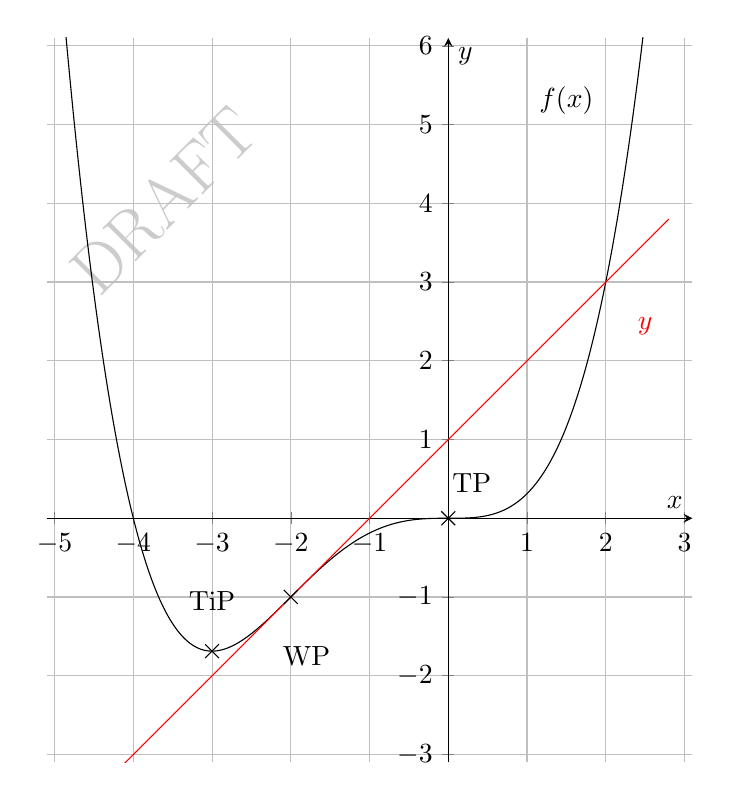
\begin{tikzpicture}
    \begin{axis}[xmin= -5.1, xmax = 3.1, ymin= -3.1, ymax=6.1,
     x=1cm,y=1cm,
        axis lines = middle, 
        ymajorgrids=true,
        xmajorgrids=true,
        xtick={-5, -4, -3,  ..., 3},
        ytick={-3, -2, ..., 6},
        xlabel = $x$,
        ylabel=$y$]
        \addplot[color= black, samples = 300, domain= -5:2.8]{1/16 * x^4 + 1/4*x^3};
        \addplot[color= red, samples = 300, domain= -4.8:2.8]{x +1};
        \draw (-3,-27/16) -- ++(-2.5pt,-2.5pt) -- ++(5pt,5pt) ++(-5pt,0pt) -- ++(5pt,-5pt);
        \draw (-3,-1.3)   node [above] {TiP};
        \draw (0,0) -- ++(-2.5pt,-2.5pt) -- ++(5pt,5pt) ++(-5pt,0pt) -- ++(5pt,-5pt);
         \draw (0.3,0.2)   node [above] {TP};
        \draw (-2,-1) -- ++(-2.5pt,-2.5pt) -- ++(5pt,5pt) ++(-5pt,0pt) -- ++(5pt,-5pt);
         \draw (-1.8,-2)   node [above] {WP};
        \draw (1.5,5)   node [above] {$f(x)$};
        \draw[red] (2.5,2.2)   node [above] {$y$};

    \end{axis}
\end{tikzpicture}}
\end{itemize}
\subsection{Platz für eigene Notizen:}
\kariert{Notizen:}{10}{11}
\section{Analytische Geometrie}
\subsection{Elementargeometrische Grundlagen}
\begin{itemize}
\item Flächeninhalt von ebenen Figuren\\
\begin{enumerate}
\item Dreieck $\longrightarrow A_{\triangle} = \frac{1}{2} \cdot g\cdot h$\\
\item Parallelogramm $\longrightarrow A_{P} = g\cdot h$\\
\item Trapez $\longrightarrow A_{T} = \frac{1}{2} \cdot (a+c)\cdot h$ hierbei sind $a$ und $c$ die Längen der Parallelen \\
\item Drachenviereck $\longrightarrow A_{\text{Drache}} = \frac{1}{2} \cdot e\cdot f$ hierbei sind $e$ und $fe$ die Längen der Diagonalen \\
\item  Kreis  $\longrightarrow A_{K} = \pi \cdot r^2$ und $U_{\text{K}} = 2\cdot \pi \cdot r$ hierbei ist $r$ der Radius des Kreises
\end{enumerate}
\item Volumen und Oberfläche von Körpern\footnote{hierbei ist $A_G$ der Flächeninhalt der Grundfläche und $h$ die Höhe}\\
\begin{enumerate}
\item Prisma $\longrightarrow V_{\text{Prisma}} = A_G \cdot h$  \\
\item Pyramide $\longrightarrow V_{\text{Pyramide}} = \frac{1}{3}\cdot A_G \cdot h$ \\
\item Zylinder $\longrightarrow V_{\text{Zylinder}} = A_G \cdot h$ und der Oberflächeninhalt eines geraden Zylinders $A_O = 2\cdot A_G + 2\cdot \pi\cdot r \cdot h$\\
\item Kegel $\longrightarrow V_{\text{Kegel}} = \frac{1}{3} \cdot A_G \cdot h$ und der Oberflächeninhalt eines geraden Kegels $A_O = A_G +  \pi\cdot r \cdot m$ mit $m $ als Länge der Mantellinie\\
\item Kugel $\longrightarrow V_{\text{Kugel}} = \frac{4}{3} \cdot \pi \cdot r^3$ und der Oberflächeninhalt $A_O = 4\cdot \pi \cdot r^2$
\end{enumerate}
\end{itemize}
\subsection{Definition von Vektoren}
\begin{itemize}
    \item Vektoren sind Pfeile im zwei - bzw. dreidimensionalen Raum
    \item Jeder Vektor ist ein Repräsentant unendlich vieler, gleich langer, gleich gerichteter und paralleler Pfeile
    \item Vektoren werden häufig durch kleine Buchstaben und einem Pfeil darüber gekennzeichnet $\vv{a}$
    \item Verläuft ein Repräsentant eines Vektors von einem Punkt z.B. $P$ zu einem zweiten Punkt z.B. $Q$, so bezeichnet man alle Repräsentanten mit $\vv{PQ}$.
    \item Werden mehrere Vektoren addiert so werden die jeweiligen Repräsentanten aneinandergereiht und das Ergebnis nennt man dann Vektorkette.
    \item Ein Vektor im 2- bzw. 3-dim. Raum wird in der Spaltenschreibweise durch 2 bzw. 3 Koordinaten beschrieben $\vv{a}= \begin{pmatrix} a_1 \\ a_2 \\ a_3 \end{pmatrix}$
    \item Der Vektor \textcolor{red}{ $\vv{0A} = \vv{A}$} bezeichnet denjenigen Vektor, der im Ursprung $0$ beginnt um im Punkt $A$ endet. Er wird als \textcolor{red}{Ortsvektor} bezeichnet.
\end{itemize}
\subsection{Spiegelungen an den Koordinatenebenen}\\[0.25cm]
Der Punkt $P(p_1|p_2|p_3)$ wird gespiegelt an
\begin{itemize}
\item $x_1x_2-$Ebene $\longrightarrow P(p_1|p_2|-p_3)$ Vorzeichen der $x_3$ Koordinaten wird geändert
\item $x_1x_3-$Ebene $\longrightarrow P(p_1|-p_2|p_3)$ Vorzeichen der $x_2$ Koordinaten wird geändert
\item $x_2x_3-$Ebene $\longrightarrow P(-p_1|p_2|p_3)$ Vorzeichen der $x_1$ Koordinaten wird geändert
\end{itemize}
\subsection{Spiegelung am Koordinatenursprung}\\[0.25cm]
Der Punkt $P(p_1|p_2|p_3)$ wird am Punkt $P(0|0|0)$ gespiegelt 
\begin{itemize}
\item $P(-p_1|-p_2|-p_3)$ bei allen Koordinaten ändern sich die \\Vorzeichen
\end{itemize}
%\vspace{0.35cm}
\subsection{Eigenschaften von Vektoren}
\begin{itemize}
\item Vektoraddition\\
\begin{enumerate}
\item $\vv{a} +\vv{b} = \vv{b} + \vv{a}$\\
\item $\left( \vv{a}+\vv{b}\right)+\vv{c} = \vv{a} +\left(\vv{b} +\vv{c}\right)$
\end{enumerate}
\item Nullvektor\\
\begin{enumerate}
\item $\vv{0} +\vv{a} = \vv{a}$ \item Der Vektor $\vv{0}$ hat die Länge $0$
\end{enumerate}
\item Gegenvektor\\
\begin{enumerate}
\item Der Vektor $-\vv{a}$ ist der Gegenvektor zu $\vv{a}$\\
\item $-\vv{a}$ ist genauso lang wir $\vv{a}$ und  zu $\vv{a}$ entgegengerichtet
\end{enumerate}
\item skalare Multiplikation\\
\begin{enumerate}
\item $\lambda \cdot \vv{a} = \lambda \cdot \begin{pmatrix} a_1 \\ a_2 \\ a_3 \end{pmatrix} = \begin{pmatrix} \lambda \cdot a_1 \\ \lambda \cdot a_2 \\ \lambda \cdot a_3 \end{pmatrix}$\\
\item Die skalare Multiplikation vervielfacht den Vektor durch den skalar $\lambda \in \mathds{R}$\\
\item Der Vektor $\lambda\cdot \vv{a}$ ist $| \lambda |-$ mal so lang wie der Vektor $\vv{a}$\\
\item Für $\lambda > 0$ hat er die gleiche Richtung wie $\vv{a}$ \\
\item Für $\lambda < 0$ hat er die entgegengesetzte Richtung wie $\vv{a}$
\end{enumerate}
\item Rechengesetze\\
\begin{enumerate}
\item Assoziativgesetz: $\lambda \cdot  \left(\mu \cdot \vv{a}\right) = \left(\lambda\cdot\mu\right)\cdot \vv{a}$\\
\item Distibutivgesetz:\\ \hspace*{0.5cm} $\lambda \cdot \left(\vv{a} + \vv{b}\right) = \lambda \cdot \vv{a}+ \lambda \cdot \vv{b}$\\ \hspace*{0.5cm} $\left(\lambda + \mu \right)\cdot \vv{a} = \lambda \cdot \vv{a} + \mu \cdot \vv{b}$
\end{enumerate}
\end{itemize}
\subsection{Rechnungen mit Vektoren}
\begin{itemize}
\item Der Verbindungsvektor $\vv{PQ}$ \\ $\vv{PQ} = \vv{Q} - \vv{P} = \begin{pmatrix} q_1 \\ q_2 \\ q_3 \end{pmatrix} - \begin{pmatrix} p_1 \\ p_2 \\ p_3 \end{pmatrix} = \begin{pmatrix} q_1 - p_1\\ q_2 - p_2\\ q_3 - p_3\end{pmatrix}$ \\ \mynote "Spitze minus Hacke"
\item Summe von Vektoren $\vv{A} +\vv{B} =  \begin{pmatrix} a_1 \\ a_2 \\ a_3 \end{pmatrix} + \begin{pmatrix} b_1 \\ b_2 \\ b_3 \end{pmatrix} = \begin{pmatrix} a_1 + b_1\\ a_2 + b_2\\ a_3 + b_3\end{pmatrix}$
\item Der Mittelpunkt der Strecke $\overline{AB}$  \\$ \longrightarrow \vv{M} = \frac{1}{2}\cdot \left(\vv{A} + \vv{B}\right)$ bestimmt 
\item Schwerpunkt des Dreiecks $\triangle ABC $\\ $\longrightarrow \vv{S}_{\text{Dreieck}} = \frac{1}{3} \left(\vv{A} + \vv{B} +\vv{C}\right)$
\item Schwerpunkt einer Pyramide $ABCS$ \\ $\longrightarrow \vv{S}_{\text{Pyramide}}= \frac{1}{4} \left(\vv{A} + \vv{B} +\vv{C} +\vv{S}\right)$
\end{itemize}
\subsection{Zusammenhang der Schwerpunkte}
\scalebox{0.8}{
\def\arraystretch{1.5}% 
\begin{tabular}{|l|c|c|}
    \hline
    & Berechnung & Teilverhältnis \\[0.2cm]
     \hline
     \hline
     Schwerpunkt einer Strecke & $\vv{S}_{AB} = \dfrac{1}{2}(\vv{A} + \vv{B})$ & 1:1\\[0.2cm]
     \hline
     Schwerpunkt eines Dreiecks &$ \vv{S}_{ABC} = \dfrac{1}{3} (\vv{A} + \vv{B} + \vv{C})$ & 1:2\\[0.2cm]
     \hline
     Schwerpunkt einer Pyramide & $\vv{S}_{ABCD} = \dfrac{1}{4}(\vv{A} + \vv{B} +\vv{C} + \vv{D})$ & 1:3\\[0.2cm]
     \hline
\end{tabular}}
\newpage
\subsection{Beispiel für Vektorketten}\\
\scalebox{0.8}{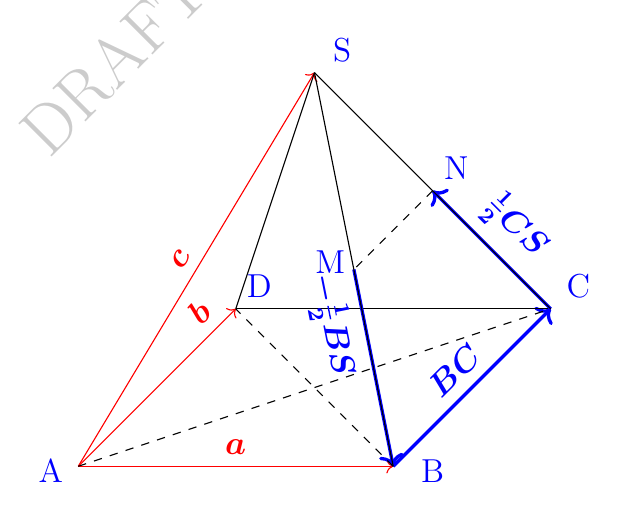
\begin{tikzpicture}[font=\boldmath]\large
    % Punkte
    \coordinate (A) at (0,0) {};
     \draw[blue] (-0.35,-0.35)   node [above] {A};
    \coordinate (B) at (4,0) {};
    \draw[blue] (4.5,-0.35)   node [above] {B};
    \coordinate (C) at (6,2) {};
    \draw[blue] (6.35,2)   node [above] {C};
    \coordinate (D) at (2,2) {};
    \draw[blue] (2.3,2)   node [above] {D};
    \coordinate (E) at (3,5) {};
    \draw[blue] (3.35,5)   node [above] {S};
    \coordinate (G) at (4.5,3.5) {};
    \draw[blue] (4.8,3.5)   node [above] {N};
    \coordinate (H) at (3.5,2.5) {};
    \draw[blue] (3.2,2.3)   node [above] {M};
    \draw[->, red]  (A) -- (B) node[sloped,midway,above] {$\vv{a}$};
    \draw[->,blue, very thick]  (B) -- (C) node[sloped,midway,above] {$\vv{BC}$};
    \draw  (C) -- (D) node[] {};
    \draw[->,red]  (A) -- (D) node[sloped,above,very near end] {$\vv{b}$};
   \draw[->,red]  (A) -- (E) node[sloped,midway,above] {$\vv{c}$};
   \draw[->,blue, very thick]  (H) -- (B) node[sloped,below, near start] {$-\frac{1}{2}\vv{BS}$};
   \draw[->,blue, very thick]  (C) -- (G) node[sloped,above, midway,] {$\frac{1}{2}\vv{CS}$};
   \draw  (E) -- (B) node[] {};
   \draw  (E) -- (C) node[] {};
   \draw  (E) -- (D) node[] {};
   \draw[dashed]  (A) -- (C) node[] {};
   \draw[dashed]  (B) -- (D) node[] {};
    \draw[dashed]  (G) -- (H) node[] {};
\end{tikzpicture} }\\
 Der Vektor $\vv{MN}$ wird mithilfe der Vektoren $\vv{a}, \vv{b}$ und $\vv{c}$ ausgedrückt.
     \begin{equation*}
            \begin{split}
                \vv{MN} &= - \dfrac{1}{2}\vv{BS} + \vv{BC} + \dfrac{1}{2} \vv{CS}\\
                &= -\dfrac{1}{2} \left( \vv{c} - \vv{a}\right) +\vv{b} + \dfrac{1}{2} \left(\vv{c} - \vv{a} -\vv{b}\right)\\
                &= -\dfrac{1}{2} \vv{c} +\dfrac{1}{2} \vv{a} +\vv{b} + \dfrac{1}{2} \vv{c} - \dfrac{1}{2}\vv{a} -\dfrac{1}{2}\vv{b}\\
                &= \dfrac{1}{2} \vv{b}
            \end{split}
        \end{equation*} 
        Damit folgt, das die Mittellinie $\overline{MN}$ parallel, gleichgerichtet aber nur halb so lang wie der Vektor $\vv{b}$ ist.
\subsection{Operationen mit Vektoren}
\begin{itemize}
\item Länge eines Vektors $\longrightarrow |\vv{a}| = \sqrt{a_1^2 + a_2^2 + a_3^2}$
\item Skalare Multiplikation $\longrightarrow \vv{b} = \lambda \cdot \vv{a} $
\item Skalarprodukt $\longrightarrow \vv{a}\circ \vv{b} = a_1\cdot b_1 + a_2\cdot b_2 + a_3\cdot b_3 \in \mathds{R}$
\item Vektorprodukt mit $\vv{a} \neq \vv{0}$ und $\vv{b} \neq \vv{0}$ \\$\longrightarrow\vv{c} = \vv{a} \times \vv{b} = \begin{pmatrix} a_1 \\a_2\\a_3\end{pmatrix} \times \begin{pmatrix} b_1 \\b_2\\b_3\end{pmatrix} = \begin{pmatrix} a_2\cdot b_3 - a_3\cdot b_2 \\a_3\cdot b_1 - a_1\cdot b_3\\a_1\cdot b_2 - a_2\cdot b_1\end{pmatrix}$
\item Spatprodukt $\longrightarrow$ Verknüpfung von Vektorprodukt und Skalarprodukt\\
\begin{enumerate}
    \item $d = \left(\vv{a} \times\vv{b}\right) \circ\vv{c} \in \mathds{R}$
\end{enumerate}
\end{itemize}
\subsection{Eigenschaften der Operationen}
\begin{itemize}
\item Länge\\
\begin{enumerate}
\item $|\vv{A}| \longrightarrow$ Abstand des Punktes $A$ vom Urpsrung\\
\item $|\vv{PQ}| \longrightarrow$ Abstand des beiden Punkte $P$ und $Q$
\end{enumerate}
\item skalare Multiplikation\\
\begin{enumerate}
\item $\lambda \vv{a} \longrightarrow$ Längenänderung von $\vv{a}$\\
\item $\vv{a}^{\ast} = \frac{1}{|\vv{a}|} \cdot \vv{a} \longrightarrow |\vv{a}^{\ast}| = 1$
\end{enumerate}
\item Skalarprodukt\\
\begin{enumerate}
\item $\vv{a}\circ \vv{b} = 0  \curvearrowright \vv{a}\perp \vv{b}$\\
\item Winkel zwischen zwei Vektoren $\vv{a}$ und $\vv{b}$\\ $\longrightarrow \cos{(\varphi)} = \frac{\vv{a} \circ \vv{b}}{|\vv{a}| \cdot |\vv{b}|} \curvearrowright \varphi = \cos^{-1}{\left(\frac{\vv{a} \circ \vv{b}}{|\vv{a}| \cdot |\vv{b}|}\right)} $
\end{enumerate}
\item Vektorprodukt\\
\begin{enumerate}
\item $\vv{a} \times \vv{b} = \vv{c}$\\
\item $\vv{a} \perp \vv{c}$ und $\vv{b} \perp \vv{c}$ \\
\item Flächeninhalt $\triangle ABC \longrightarrow A_{\text{Dreieck}} = \frac{1}{2} \cdot | \vv{a}\times \vv{b}|$\\
\item Flächeninhalt Parallelogramm $\longrightarrow A_{\text{P}} = |\vv{a} \times \vv{b}|$
\end{enumerate}
\item Spatprodukt $\longrightarrow$ bestimmt ein Volumen\\
\begin{enumerate}
    \item Volumen eines Spates $\longrightarrow V_{\text{Spat}} = |\left(\vv{AB} \times \vv{AD} \right)\circ\vv{AE}|$\\
    \scalebox{0.8}{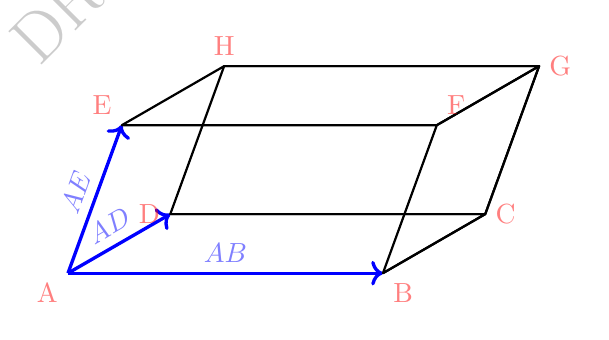
\begin{tikzpicture}
 \begin{scope}[
    x={(4cm,0cm)},
    y={({cos(30)*1.5cm},{sin(30)*1.5cm})},
    z={({cos(70)*2cm},{sin(70)*2cm})},
    line join=round,fill opacity=0.5,thick]

  % Ecken definieren
  \coordinate (A) at (0,0,0);
  \coordinate (B) at (1,0,0);
  \coordinate (C) at (1,1,0);
  \coordinate (D) at (0,1,0);
  \coordinate (E) at (0,0,1);
  \coordinate (F) at (1,0,1);
  \coordinate (G) at (1,1,1);
  \coordinate (H) at (0,1,1);
%Vektoren zeichnen
\draw[->,blue, very thick]  (A) -- (B) node[sloped,above,midway] {$\vv{AB}$};
\draw[->,blue, very thick]  (A) -- (D) node[sloped,above,midway] {$\vv{AD}$};
\draw[->,blue, very thick]  (A) -- (E) node[sloped,above,midway] {$\vv{AE}$};
 \draw[] (B) -- (C) -- (D);
  
  % Flächen zeichnen
  %\draw[] (A) -- (B) -- (C) -- (D) -- cycle;
  \draw[] (D) -- (C) -- (G) -- (H) -- cycle;
  \draw[] (B) -- (F) -- (G) -- (C) -- cycle;
%  \draw[] (A) -- (E) -- (F) -- (B) -- cycle;
 % \draw[] (A) -- (D) -- (H) -- (E) -- cycle;
  \draw[] (E) -- (F) -- (G) -- (H) -- cycle;

  % Punkte beschriften
  \foreach \name/\pos in {
    A/below left,
    B/below right,
    C/right,
    D/left,
    E/above left,
    F/above right,
    G/right,
    H/above}
    \draw[red] (\name) node[\pos] {\name};

 \end{scope}
\end{tikzpicture}}\\
    \item Volumen einer dreiseitigen Pyramide\\ $ \longrightarrow V_{\text{Pyramide}}= |\frac{1}{6}\cdot \left(\vv{AB} \times \vv{AC} \right)\circ\vv{AS}| $\\
    \scalebox{0.9}{%
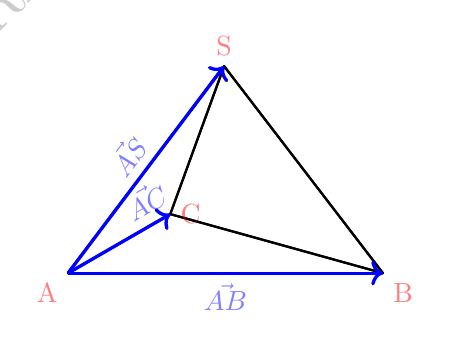
\begin{tikzpicture}
 \begin{scope}[
    x={(4cm,0cm)},
    y={({cos(30)*1.5cm},{sin(30)*1.5cm})},
    z={({cos(70)*2cm},{sin(70)*2cm})},
    line join=round, fill opacity=0.5, thick]

  % Eckpunkte definieren
  \coordinate (A) at (0,0,0);    % Basisdreieck
  \coordinate (B) at (1,0,0);
  \coordinate (C) at (0,1,0);
  \coordinate (S) at (0,1,1); % Spitze

  % Flächen der Pyramide
  \draw[] (A) -- (B) -- (C) -- cycle; % Basis
  \draw[] (A) -- (B) -- (S) -- cycle;
  \draw[] (B) -- (C) -- (S) -- cycle;
  \draw[] (C) -- (A) -- (S) -- cycle;

  % Vektoren einzeichnen
  \draw[->,blue, very thick] (A) -- (B) node[sloped,midway, below] {$\vec{AB}$};
  \draw[->,blue, very thick] (A) -- (C) node[sloped,very near end, above] {$\vec{AC}$};
  \draw[->,blue, very thick] (A) -- (S) node[sloped,midway, above, thick] {$\vec{AS}$};

  % Punkte beschriften
  \draw[red] (A) node[below left] {A};
  \draw[red] (B) node[below right] {B};
  \draw[red] (C) node[right] {C};
  \draw[red] (S) node[above] {S};

 \end{scope}
\end{tikzpicture}%
}
\end{enumerate}
\end{itemize}
\subsection{Kugelgleichung}
\begin{itemize}
\item Kugel um den Ursprung mit Radius $r$\\$\longrightarrow \left(x_1\right)^2 +\left(x_2 \right)^2+\left(x_3 \right)^2 = r^2$ 
\item  Kugel um $M(m_1|m_2|m_3)$ mit Radius $r$\\$ \longrightarrow \left(x_1 -m_1\right)^2 +\left(x_2 -m_2\right)^2+\left(x_3 -m_3\right)^2 = r^2 $  
\end{itemize}
\subsection{Platz für eigene Notizen:}
\kariert{Notizen:}{10}{17}
\section{Stochastik}
\subsection{Ereignisalgebra}
\begin{itemize}
    \item Ein \textcolor{red}{Ereignis} A ist eine Teilmenge des \textcolor{red}{Ergebnisraums} $\Omega$
    \item Ein Ereigni A \textcolor{red}{tritt ein}, wenn das \textcolor{red}{Versuchsergebnis} $\omega$ in A enthalten ist, es gilt also $\omega \in A$
    \item Alle Elemente von $\Omega$ sie nicht zum Ereignis A gehören, fasst man unter dem Namen \textcolor{red}{Gegenereignis} $\overline{A}$ zusammen, es gilt $\overline{A}= \Omega\setminus A$
    \item Zwei Ereignisse A und B heißen \textcolor{red}{unvereinbar}, wenn gilt \\$A \cap B = \{ \hspace{0.15cm}\}$.
\end{itemize}
\subsection{Venn-Diagramme}
\begin{itemize}
    \item Gegenereignis $\bar{A}$: "nicht A", Ereignis A tritt nicht ein\\
    \scalebox{0.8}{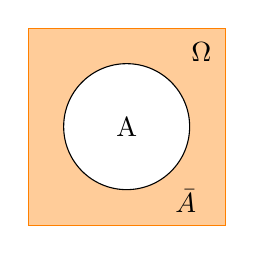
\begin{tikzpicture}
\draw[orange, fill=orange!40] (0,0) rectangle (2.5,2.5);
\begin{scope}
    \clip (0,0) rectangle (2.5,2.5);
    \fill[white] (1.25,1.25) circle (0.8);
    \draw (1.25,1.25) circle (0.8);
\end{scope}
\node at (2.2,2.2) {$\Omega$};
\node at (1.25,1.25) {A};
\node at (2,0.3) {$\bar{A}$};
\end{tikzpicture}}
\item Vereinigungsmenge $A \cup B$: "A oder B",  Mindestens eines der beiden Ereignisse tritt ein \\ \scalebox{0.8}{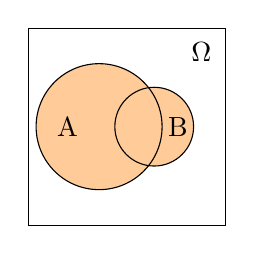
\begin{tikzpicture}
\draw (0,0) rectangle (2.5,2.5);
\fill[orange!40] (0.9,1.25) circle (0.8);
\fill[orange!40] (1.6,1.25) circle (0.5);
\draw (0.9,1.25) circle (0.8);
\draw (1.6,1.25) circle (0.5);
\node at (2.2,2.2) {$\Omega$};
\node at (0.5,1.25) {A};
\node at (1.9,1.25) {B};
\end{tikzpicture}}
\item Schnittmenge $A \cap B$:  "A und B", Beide Ereignisse treten ein \\ 
\scalebox{0.8}{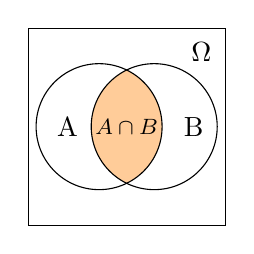
\begin{tikzpicture}
\draw (0,0) rectangle (2.5,2.5);
\begin{scope}
    \clip (0.9,1.25) circle (0.8);
    \fill[orange!40] (1.6,1.25) circle (0.8);
\end{scope}
\draw (0.9,1.25) circle (0.8);
\draw (1.6,1.25) circle (0.8);
\node at (2.2,2.2) {$\Omega$};
\node at (0.5,1.25) {A};
\node at (2.1,1.25) {B};
\node at (1.25,1.25) {\footnotesize{$A\cap B$}};
\end{tikzpicture}}
\item "A und nicht B" $A \cap \overline{B}$: Es tritt genau das Ereignis A ein\\
\scalebox{0.8}{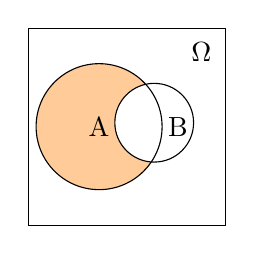
\begin{tikzpicture}
\draw (0,0) rectangle (2.5,2.5);
\fill[orange!40] (0.9,1.25) circle (0.8);
\begin{scope}
    \clip (1.6,1.3) circle (0.5);
    \fill[white] (0.9,1.25) circle (0.8);
\end{scope}
\draw (0.9,1.25) circle (0.8);
\draw (1.6,1.3) circle (0.5);
\node at (2.2,2.2) {$\Omega$};
\node at (0.9,1.25) {A};
\node at (1.9,1.25) {B};
\end{tikzpicture}}

\item "nicht A und nicht B" $\bar{A} \cap \bar{B} = \overline{A\cup B}$: Weder A noch B tritt ein\\ \scalebox{0.8}{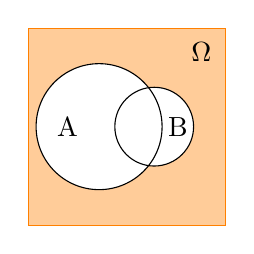
\begin{tikzpicture}
\draw[orange, fill=orange!40] (0,0) rectangle (2.5,2.5);
\begin{scope}
    \clip (0,0) rectangle (2.5,2.5);
    \fill[white] (0.9,1.25) circle (0.8);
    \fill[white] (1.6,1.25) circle (0.5);
    \draw (0.9,1.25) circle (0.8);
    \draw (1.6,1.25) circle (0.5);
\end{scope}
\node at (2.2,2.2) {$\Omega$};
\node at (0.5,1.25) {A};
\node at (1.9,1.25) {B};
\end{tikzpicture}}
\item "nicht A oder nicht B" $\bar{A} \cup \overline{B} = \overline{A \cap B}$: Höchstens eines der Ereignisse tritt ein \\ 
\scalebox{0.8}{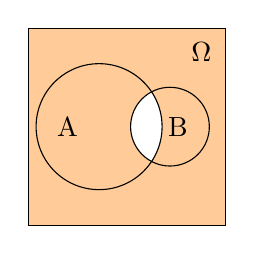
\begin{tikzpicture}
% Rechteck als Hintergrund orange
\fill[orange!40] (0,0) rectangle (2.5,2.5);

% Schnittmenge beider Kreise weiß machen
\begin{scope}
  \clip (0.9,1.25) circle (0.8);          % zuerst auf Kreis A beschränken
  \fill[white] (1.8,1.25) circle (0.5);   % dann innerhalb von A Kreis B füllen
\end{scope}

% Kreislinien zeichnen
\draw (0.9,1.25) circle (0.8);
\draw (1.8,1.25) circle (0.5);

% Rechteckrahmen zeichnen
\draw (0,0) rectangle (2.5,2.5);

% Beschriftungen
\node at (2.2,2.2) {$\Omega$};
\node at (0.5,1.25) {A};
\node at (1.9,1.25) {B};
\end{tikzpicture}}
\end{itemize}
\subsection{Laplace-Wahrscheinlichkeiten}
\begin{itemize}
    \item Alle Ergebnisse eines Zufallsexperiments sind gleich wahrscheinlich
    \item Beispiel:
    \begin{enumerate}
        \item drehen eines Glücksrads mit gleich großen Sektoren
        \item "normaler" Würfel
        \item Wurf mit einer "normalen" Münze
    \end{enumerate}
    \item Die Wahrscheinlichkeit eines Ereignisses A ist gleich der Anzahl der Elemente von A dividiert durch die Anzahl der Elemente von $\Omega$
    \item $P(A) = \frac{|A|}{|\Omega |} = \frac{\text{Anzahl der günstigen Ergebnisse}}{\text{Anzahl der möglichen Ergebnisse}}$
    \item $|A|$ entspricht der Mächtigkeit von A
    \item $|\Omega|$ entspricht der Mächtigkeit von $\Omega$
\end{itemize}
\subsection{Axiomatischer Aufbau der Stochastik}\\
Eine Funktion P, die jedem Ereignis $A$ eine reelle Zahl $P(A)$ zuordnet, heißt \textcolor{red}{Wahrscheinlichkeitsverteilung}, wenn sie die folgenden Eigenschaften besitzt: 
\begin{itemize}
    \item Axiom I: $P(A) \geq 0$
    \item Axiom II: $P(\Omega) = 1$ 
    \item Axiom III: $A\cap B = \{ \hspace{0.15cm} \} \Rightarrow P(A\cup B) = P(A) + P(B)$  wenn die Schnittmenge zweier Ereignisse leer ist, dann gilt für die Wahrscheinlichkeit der Vereinigung zweier Ereignisse \\$P(A\cup B) = P(A) + P(B)$ 
\end{itemize}
\subsubsection{Eigenschaften}
\begin{itemize}
    \item $P(A) + P(\bar{A}) = 1$
    \item $P(\{ \hspace{0.15cm} \}) = 0 $
    \item $A\subseteq B \Rightarrow  P(A) \leq P(B)$
    \item $P(A) \leq 1$ mit $A\subseteq \Omega$
    \item $P(A \cup B) = P(A) + P(B) - P(A\cap B)$
\end{itemize}
\subsection{Bedingte Wahrscheinlichkeit}\\
Ist das Ereignis A eingetreten, dann ist die \textcolor{red}{bedingte Wahrscheinlichkeit} für das Eintreten eines Ereignisses B gleich \\$P_A(B) = \dfrac{P(A \cap B)}{P(A)}$. Folgt aus der Anwendung der Pfadregeln.\\
\scalebox{0.65}{
% allgemeines Layout des Baums
\tikzstyle{level 1}=[level distance=2.5cm, sibling distance=5cm]
\tikzstyle{level 2}=[level distance=2.5cm, sibling distance=2.5cm]
% definiert Knoten- und Endpunkte
% text width ändert die Boxbreite wobei 1em einem Zeichen entspricht
\tikzstyle{bag} = [circle, draw, text width=1em, inner sep=2pt, text centered]
\tikzstyle{end} = [circle, minimum width=5pt, fill, inner sep=0pt]
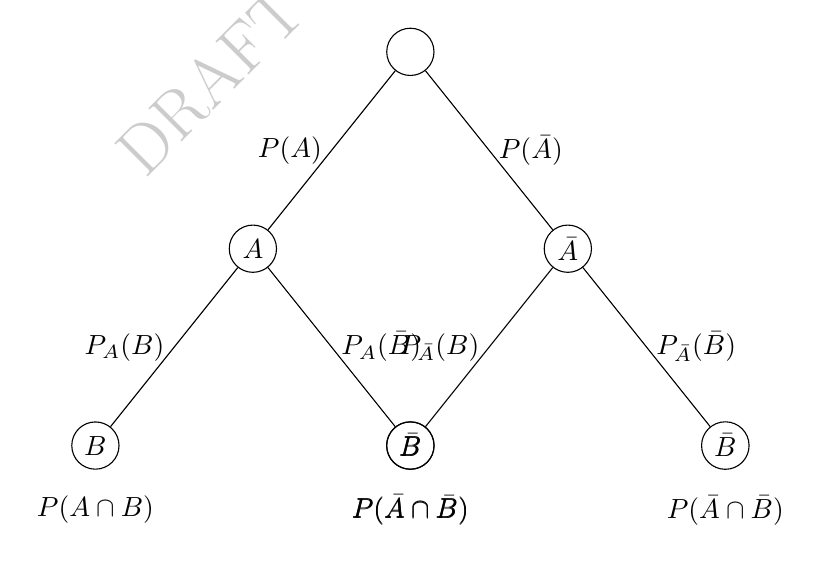
\begin{tikzpicture}[grow=down, sibling distance=4cm, level distance=2.5cm]
  \tikzset{bag/.style={circle, draw=black, minimum size=6mm, inner sep=2pt}}

  \node[bag] {}
  child {
    node (A) [bag] {$A$}
    child {
      node (AB) [bag] {$B$}
      edge from parent
        node[left] {$P_{A}(B)$}
    }
    child {
      node (AnB) [bag] {$\bar{B}$}
      edge from parent
        node[right] {$P_{A}(\bar{B})$}
    }
    edge from parent
      node[left] {$P(A)$}
  }
  child {
    node (nA) [bag] {$\bar{A}$}
    child {
      node (nAB) [bag] {$B$}
      edge from parent
        node[left] {$P_{\bar{A}}(B)$}
    }
    child {
      node (nAnB) [bag] {$\bar{B}$}
      edge from parent
        node[right] {$P_{\bar{A}}(\bar{B})$}
    }
    edge from parent
      node[right] {$P(\bar{A})$}
  };

  % Pfad-Wahrscheinlichkeiten direkt unter den Knoten
  \node[below=2mm of AB]   {$P(A \cap B)$};
  \node[below=2mm of AnB]  {$P(A \cap \bar{B})$};
  \node[below=2mm of nAB]  {$P(\bar{A} \cap B)$};
  \node[below=2mm of nAnB] {$P(\bar{A} \cap \bar{B})$};

\end{tikzpicture}
}

Nach der ersten Pfadregel berechnet sich die Wahrscheinlichkeit $P(A\cap B)$ durch das Produkt der einzelnen Pfadwahrscheinlichkeiten. Es gilt damit also $P(A\cap B) = P(A) \cdot P_{A}(B)$ und daraus folgt die Beziehung: $P_{A}(B) = \dfrac{P(A \cap B)}{P(A)}$
\subsubsection{Stochastische Unabhängigkeit}\\
Zwei Ereignisse $A$ und $B$ heißen \textcolor{red}{stochastisch unabhängig}, wenn $P(A \cap B) = P(A)\cdot P(B)$ gilt. Andernfalls nennt man diese \textcolor{red}{stochastisch abhängig}.
\subsection{Kombinatorik}\\
\begin{enumerate}
    \item Permutation als  Anordnung von $n$ Objekten in einer bestimmten Reihenfolge $\longrightarrow n! = n\cdot ( n-1) \cdot (n-2)\cdot \ldots \cdot 3\cdot  2\cdot 1$\\
    \item Unterscheidungsmöglichkeiten in einem Urnenexperimentes: Man zieht aus einer Menge mit $n$ Elementen $k-$Elemente heraus\\
    \begin{tabular}{|c||c|c|}
    \hline
         &  Mit Reihenfolge & Ohne Reihenfolge\\
           \hline\hline
     Mit Zurücklegen   & $n^k$ & $\binom{n+k-1}{k}$\\
     \hline
     Ohne Zurücklegen & $\frac{n!}{\left(n-k\right)!}$& $\binom{n}{k} = \frac{n!}{k!\left(n-k\right)!}$\\
     \hline
    \end{tabular} 
\end{enumerate}
\begin{itemize}
\item Eigenschaften des Binomialkoeffizienten
\end{itemize}
\begin{enumerate}
    \item Der Binomialkoeffizient ist symmetrisch $\longrightarrow \binom{n}{k} = \binom{n}{n-k}$\\
    \item Besondere Werte des Binomialkoeffizienten $\binom{n}{0}= 1; \binom{n}{1} = n$ und $\binom{n}{n}=1$
\end{enumerate}
\newpage
\subsection{Zufallsgrößen}
\begin{itemize}
    \item Eine Funktion $X$, die jedem Ergebnis $\omega$ eines Ergebnisraumes $\Omega$ eine reelle Zahl $x$ zuordnet, heißt \textcolor{red}{Zufallsgröße\footnote{Zufallsgröße $\longrightarrow$ ZG}} X.
    \item Jeder Wert $x$ einer ZG $X$ tritt mit einer bestimmten Wahrscheinlichkeit $P(X=x)$ auf. Die Funktion, die jedem Wert $x$ einer ZG $X$ die Wahrscheinlichkeit $P(X=x)$ zuordnet, heißt \textcolor{red}{Wahrscheinlichkeitsverteilung} der ZG $X$.
     \item Als Beispiel ist hier $P(X=4) = 0,2$ dargestellt.
   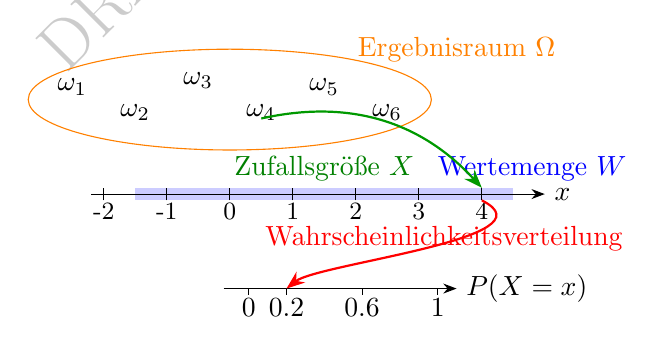
\begin{tikzpicture}[>=Stealth, scale=0.8]

% Ergebnisraum Omega (kompakter)
\draw[orange] (0,4.5) ellipse (3.2cm and 0.8cm);
\node[orange] at (3.6,5.3) {Ergebnisraum $\Omega$};
\foreach \i/\x/\y in {
  \omega_1/-2.5/4.7,
  \omega_2/-1.5/4.3,
  \omega_3/-0.5/4.8,
  \omega_4/ 0.5/4.3,
  \omega_5/ 1.5/4.7,
  \omega_6/ 2.5/4.3
}{
  \node at (\x,\y) {\(\i\)};
}

% Wertemenge W
% Blauer Hintergrund unter Achse von 1.5 bis 12
\fill[blue!20] (-1.5,2.9) rectangle (4.5,3.1);
\draw[->] (-2.2,3) -- (5,3) node[right] {$x$};
\foreach \x in {-2,-1,0,1,2,3,4}
  \draw (\x,2.9) -- (\x,3.1) node[below=2pt] {\small \x};
\node[blue] at (4.8,3.4) {Wertemenge $W$};

% Grüner Pfeil: Zufallsgröße X
\draw[->, thick, green!60!black] (0.5,4.2) to[bend left=30] (4,3.1);
\node[green!50!black] at (1.5,3.4) {Zufallsgröße $X$};

% P(X = x)-Achse
\draw[->] (-0.1,1.5) -- (3.6,1.5) node[anchor=west] {$P(X = x)$};

% Tick-Marken und Beschriftungen
\foreach \i/\label in {0/0, 1/0.2,  3/0.6, 5/1} {
  \draw (\i*0.6 + 0.3,1.5) -- ++(0,-0.1); % Markierung
  \node at (\i*0.6 + 0.3,1.2) {\label};   % Beschriftung
}

% Roter Pfeil: zweifach gebogen und zeigt exakt auf 0.2 (bei x=0.9, y=1.5)
\draw[->, thick, red]
  (4,2.9) .. controls (5.2,2.3) and (1.4,1.9) .. (0.9,1.5);

\node[red] at (3.4,2.3) {Wahrscheinlichkeitsverteilung};
\end{tikzpicture}
  
\end{itemize}
\subsubsection{Erwartungswert und Varianz}
\begin{itemize}
    \item Eine ZG nimmt die Werte $x_1, x_2,\ldots , x_n$ mit den Wahrscheinlichkeiten $P(X=x_1), P(X=x_2), \ldots, P(X=x_n)$ an. Dann heißt der zu erwartende Mittelwert\\ $ \mu =E(X) = \sum\limits_{i=1}^n x_i\cdot P(X=x_i) \\= x_1\cdot P(X=x_1) + x_2\cdot P(X=x_2) +\ldots + x_n \cdot P(X=x_n)$ \textcolor{red}{Erwartungswert} von $X$. \mynote Der Erwartungswert $\mu$ ist häufig \textcolor{red}{kein} Wert, den die ZG annimmt.
    \item Eine ZG mit $E(X) = \mu$ nehme die Werte $x_1, x_2,\ldots , x_n$ mit den Wahrscheinlichkeiten\\ $P(X=x_1), P(X=x_2), \ldots, P(X=x_n)$ an. Dann heißt die mittlere quadratische Abweichung von $\mu$ \textcolor{red}{Varianz} von $X$: \\ $Var(X) = \sum\limits_{i=1}^n \left(x_i - \mu\right)^2 \cdot P(X = x_i)\\ = \left(x_1 - \mu\right)^2 \cdot P(X = x_1) + \ldots + \left(x_n - \mu\right)^2 \cdot P(X = x_n)$
    \item Die Standardabweichung $\sigma$ einer ZG $X$ bestimmt sich durch $\sigma = \sqrt{Var(X)}$
\end{itemize}

\subsection{Hypergeometrische Verteilung}
\begin{itemize}
    \item Als Anwendung der Kombinatorik mit den Einschränkungen \textcolor{red}{ziehen ohne zurücklegen} und \textcolor{red}{ohne Beachtung der Reihenfolge}
    \item Es gibt $\binom{n}{k}$ Möglichkeiten $k$ Objekte ohne Berücksichtigung der Reihenfolge aus $n$ verschiedenen Objekten auszuwählen.
    \item Aus einer Urne mit $N$ Kugeln, wovon $S$ schwarz sind, werden $n$ Kugeln ohne Zurücklegen gezogen. Die ZG $X$ beschreibt die Anzahl der gezogenen schwarzen Kugeln.\\
Wahrscheinlichkeitsverteilung dieser Zufallsgröße \\$P(X = k) = \dfrac{\binom{S}{k}\cdot \binom{N-S}{n-k}}{\binom{N}{n}}$ mit $k\leq n$ und $k\leq S$
\item Beispiel: 
\begin{enumerate}
\item $N=200$ , $S = 10$, $n=180$ und $k=9$\\
    \item $P(X=9)= \dfrac {\binom{10}{9} \cdot \binom {190}{171}}{\binom{200}{180}} \approx 39,74\%$
\end{enumerate}
\end{itemize}
\subsection{Binomialverteilung}
\subsubsection{Bernoulli-Kette}
\begin{itemize}
    \item Ein ZG mit nur zwei möglichen Ergebnissen nennt man Bernoulli-Experiment $ \longrightarrow$ Treffer "1" bzw. Niete "0"
    \item Trefferwahrscheinlichkeit $p$
    \item Nietenwahrscheinlichkeit $q = 1-p$
    \item Wird ein Bernoulli-Experiment $n-$mal unabhängig durchgeführt, spricht man von einer \textcolor{red}{Bernoulli-Kette} der \textcolor{red}{Länge n}. 
    \item Die Trefferwahrscheinlichkeit $p$ bleibt dabei konstant \\$\longrightarrow$ ziehen ohne zurücklegen ohne Beachtung der Reihenfolge
    \item Beispiel\\
    % allgemeines Layout des Baums
\tikzstyle{level 1}=[level distance=2.5cm, sibling distance=5cm]
\tikzstyle{level 2}=[level distance=2.5cm, sibling distance=2.5cm]
% definiert Knoten- und Endpunkte
% text width ändert die Boxbreite wobei 1em einem Zeichen entspricht
\tikzstyle{bag} = [circle, draw, text width=1em, inner sep=2pt, text centered]
\tikzstyle{end} = [circle, minimum width=5pt, fill, inner sep=0pt]
\scalebox{0.55}{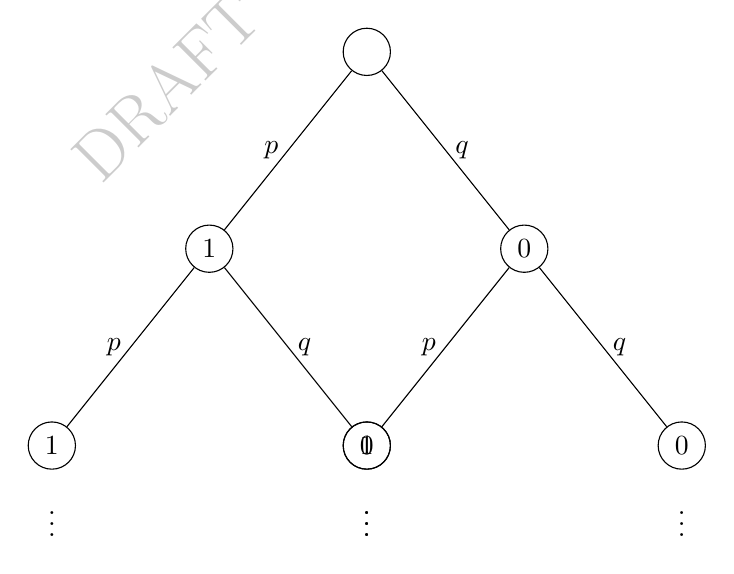
\begin{tikzpicture}[grow=down, sibling distance=4cm, level distance=2.5cm]
  \tikzset{bag/.style={circle, draw=black, minimum size=6mm, inner sep=2pt}}

  \node[bag] {}
  child {
    node (A) [bag] {$1$}
    child {
      node (AB) [bag] {$1$}
      edge from parent
        node[left] {$p$}
    }
    child {
      node (AnB) [bag] {$0$}
      edge from parent
        node[right] {$q$}
    }
    edge from parent
      node[left] {$p$}
  }
  child {
    node (nA) [bag] {$0$}
    child {
      node (nAB) [bag] {$1$}
      edge from parent
        node[left] {$p$}
    }
    child {
      node (nAnB) [bag] {$0$}
      edge from parent
        node[right] {$q$}
    }
    edge from parent
      node[right] {$q$}
  };

  % Pfad-Wahrscheinlichkeiten direkt unter den Knoten
  \node[below=2mm of AB]   {$\vdots$};
  \node[below=2mm of AnB]  {$\vdots$};
  \node[below=2mm of nAB]  {$\vdots$};
  \node[below=2mm of nAnB] {$\vdots$};

\end{tikzpicture}}
\end{itemize}
\subsubsection{Wahrscheinlichkeiten}
\begin{itemize}
    \item Wahrscheinlichkeit eines Ergebnisses $\omega$ in einer Bernoulli-Kette $\longrightarrow$ Wahrscheinlichkeit entlang eines Astes\\ $P_p^n(\omega) = \underbrace{p^k}_{\shortstack{\textcolor{red}{\footnotesize{Treffer-}}\\ \textcolor{red}{\footnotesize{wahrscheinlichkeit}}}} \cdot
\underbrace{(1 - p)^{n - k}}_{\shortstack{\footnotesize{\textcolor{red}{Nieten-}}\\ \footnotesize{\textcolor{red}{wahrscheinlichkeit}}}}$\\
    \item Wahrscheinlichkeit für \textcolor{red}{genau k} Treffer beträgt\\ $P_p^n(X = k) = \underbrace{\binom{n}{k}}_{\shortstack{\textcolor{red}{\footnotesize{Anzahl der Pfade}}\\ \textcolor{red}{\footnotesize{mit $k$ Treffern}}}} \underbrace{p^k}_{\shortstack{\textcolor{green}{\footnotesize{Treffer-}}\\ \textcolor{green}{\footnotesize{wahrscheinlichkeit}}}} \cdot
\underbrace{(1 - p)^{n - k}}_{\shortstack{\footnotesize{\textcolor{blue}{Nieten-}}\\ \footnotesize{\textcolor{blue}{wahrscheinlichkeit}}}}$\\
    \item Mindestens ein Treffer\\ $P_p^n(X\geq 1) = 1- P_p^n(X=0) =1-q^n$\\
    \item Anwendung der Wahrscheinlichkeiten $\longrightarrow$ 3m$-$ Aufgaben\\
\begin{enumerate}
    \item Mindest-Trefferwahrscheinlichkeit $p$ bei gegebenem $n$
    \begin{equation*}
        \begin{split}
            P^5_p(X\geq 1) &\geq 0,9\\
            1-P^5_p(X=0)&\geq 0,9\\
            1-(1-p)^5 &\geq 0,9\\
            p\geq \sqrt[5]{0,1}
        \end{split}
    \end{equation*}
    \item Mindest-Anzahl an Versuchen $n$ bei gegebenem $p$
    \begin{equation*}
        \begin{split}
            P^n_{0,6}(X\geq 1) &\geq 0,999\\
            1-P^n_{0,6}(X=0)&\geq 0,999\\
            1-(0,4)^n &\geq 0,999\\
           n\geq \frac{\ln{(0,001)}}{\ln{(0,4)}}
        \end{split}
    \end{equation*}
\end{enumerate}
\end{itemize}
\subsubsection{Erwartungswert und Varianz}
\begin{itemize}
    \item Wahrscheinlichkeitsverteilung eine Binomialverteilung\\
    \begin{enumerate}
        \item $B(n,p) = P_p^n(X=k) = \binom{n}{k} \cdot p^k \cdot q^{n-k}$ mit\\ $k\in \{0, 1, \ldots, n\}$\\
        \item kumulative Verteilung:\\ $F_p^n(k) = P_p^n(X\leq k)=\sum\limits_{i=0}^k P_p^n(X=k)\\ =\sum\limits_{i=0}^k \binom{n}{k} \cdot p^k \cdot q^{n-k}$ mit $k\in \{0, 1, \ldots, n\}$
    \end{enumerate}
    \item Erwartungswert: $E(X) = n\cdot p$
    \item Varianz: $Var(X)= n\cdot p \cdot q$
    \item Standardabweichung: $\sigma = \sqrt{Var(x)} = \sqrt{n\cdot p \cdot q}$
\end{itemize}

\end{document}